\documentclass[12pt, a4paper, oneside]{article}\usepackage[]{graphicx}\usepackage[]{color}
%% maxwidth is the original width if it is less than linewidth
%% otherwise use linewidth (to make sure the graphics do not exceed the margin)
\makeatletter
\def\maxwidth{ %
  \ifdim\Gin@nat@width>\linewidth
    \linewidth
  \else
    \Gin@nat@width
  \fi
}
\makeatother

\definecolor{fgcolor}{rgb}{0.345, 0.345, 0.345}
\newcommand{\hlnum}[1]{\textcolor[rgb]{0.686,0.059,0.569}{#1}}%
\newcommand{\hlstr}[1]{\textcolor[rgb]{0.192,0.494,0.8}{#1}}%
\newcommand{\hlcom}[1]{\textcolor[rgb]{0.678,0.584,0.686}{\textit{#1}}}%
\newcommand{\hlopt}[1]{\textcolor[rgb]{0,0,0}{#1}}%
\newcommand{\hlstd}[1]{\textcolor[rgb]{0.345,0.345,0.345}{#1}}%
\newcommand{\hlkwa}[1]{\textcolor[rgb]{0.161,0.373,0.58}{\textbf{#1}}}%
\newcommand{\hlkwb}[1]{\textcolor[rgb]{0.69,0.353,0.396}{#1}}%
\newcommand{\hlkwc}[1]{\textcolor[rgb]{0.333,0.667,0.333}{#1}}%
\newcommand{\hlkwd}[1]{\textcolor[rgb]{0.737,0.353,0.396}{\textbf{#1}}}%

\usepackage{framed}
\makeatletter
\newenvironment{kframe}{%
 \def\at@end@of@kframe{}%
 \ifinner\ifhmode%
  \def\at@end@of@kframe{\end{minipage}}%
  \begin{minipage}{\columnwidth}%
 \fi\fi%
 \def\FrameCommand##1{\hskip\@totalleftmargin \hskip-\fboxsep
 \colorbox{shadecolor}{##1}\hskip-\fboxsep
     % There is no \\@totalrightmargin, so:
     \hskip-\linewidth \hskip-\@totalleftmargin \hskip\columnwidth}%
 \MakeFramed {\advance\hsize-\width
   \@totalleftmargin\z@ \linewidth\hsize
   \@setminipage}}%
 {\par\unskip\endMakeFramed%
 \at@end@of@kframe}
\makeatother

\definecolor{shadecolor}{rgb}{.97, .97, .97}
\definecolor{messagecolor}{rgb}{0, 0, 0}
\definecolor{warningcolor}{rgb}{1, 0, 1}
\definecolor{errorcolor}{rgb}{1, 0, 0}
\newenvironment{knitrout}{}{} % an empty environment to be redefined in TeX

\usepackage{alltt} % Paper size, default font size and one-sided paper
%\graphicspath{{./Figures/}} % Specifies the directory where pictures are stored
%\usepackage[dcucite]{harvard}
\usepackage{rotating}
\usepackage{amsmath}
\usepackage{setspace}
\usepackage{pdflscape}
\usepackage[flushleft]{threeparttable}
\usepackage{multirow}
\usepackage[comma, sort&compress]{natbib}% Use the natbib reference package - read up on this to edit the reference style; if you want text (e.g. Smith et al., 2012) for the in-text references (instead of numbers), remove 'numbers' 
\usepackage{graphicx}
%\bibliographystyle{plainnat}
\bibliographystyle{agsm}
\usepackage[colorlinks = true, citecolor = blue, linkcolor = blue]{hyperref}
%\hypersetup{urlcolor=blue, colorlinks=true} % Colors hyperlinks in blue - change to black if annoying
%\renewcommand[\harvardurl]{URL: \url}
\IfFileExists{upquote.sty}{\usepackage{upquote}}{}
\begin{document}
\title{The Investment Problem}
\author{Rob Hayward}
\maketitle
\section{Introduction}
The first step in the Investment Case Study is to identify the Investment Problem. This will involve five main steps:
\begin{enumerate}
\item Identify the assets and liabilities of the client
\item Calculate and project forward the income and expenses of the client
\item Outline the goals of the client
\item Assess the level of risk that the client would be willing to take
\end{enumerate}

\section{Identify the assets and liabilities of the client}
You have been told some details of the client that you will advise.  They may own a house or a car.  If you do not have information about something, you can make an assumption.  At the end of the process you should have a balance sheet that outlines the assets and liabilities of the client.  This will tell you their \emph{net worth}; it will let you assess how much money could be raised through the sale of assets; it will identify the liabilities that will have to be covered by income or asset sales.  Don't forget the inheritance. 

\section{Calculate and project forward the income and expenses}
You have some information about the current income and expenses of the client. Once you have the basis income, you make an assessment of the expenses that they face.  You can assume that you have asked them to fill out a questionnaire. Take the expenses from the income to give an estimate of the spare cash.  This may be a negative number.  

Now project this forward.  You will have to make some assumptions about the increase in wages and the adjustments that will be made if they change job or retire.  You will also have to project the increase in cost of their expenses. This will leave you with an estimate of how much spare money will be available each year. 

\section{Outline the goals of the client}
You have been given very clear instructions about the goals of the client.  What do they want to achieve?  You have a picture of the assets and liabilities, you have a projection of the income and expenses each year, you now have to add the goals to your timeline so that it is clear what they want to achieve at each date.  You must estimate the cost of the goals.  This will leave you with an answer to the question - 

How much money do they need and which year do they need it?

\section{Assess the level of risk that the client would be willing to take}
Risk is a difficult concept.  Some of you have already looked at this in the literature review.  

Risk tolerance is determined by a number of factors:
\begin{enumerate}
\item Age
\item Personalisty
\item Income
\item Culture
\item Investment goals
\end{enumerate}

In reality, investment advisors would get their customers to complete a questionnaire that would provide some means of assessing their willingness to take risk.  

\subsection{Liquidity risk}
Onc very important risk that firms will have to face is \emph{liqudity risk}.  This is the risk that you will have to sell the asset for price that is very different from what you bought it for.  This increases as the date of the goal approaches.  For example, people retiring in 2008 with a retirement fund full of equities would have a much smaller pension that someone retiring in 2006 because of the sharp fall in equity prices that was experienced in that time.

\begin{knitrout}
\definecolor{shadecolor}{rgb}{0.969, 0.969, 0.969}\color{fgcolor}
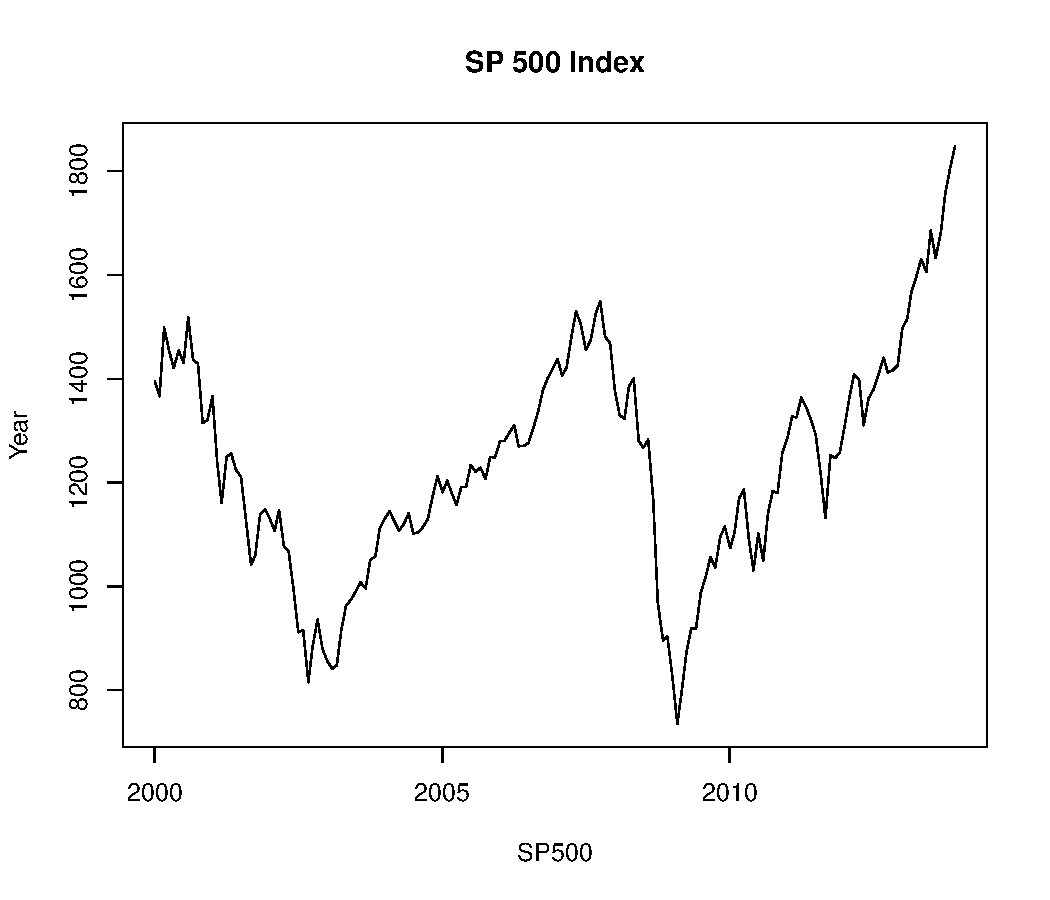
\includegraphics[width=\maxwidth]{figure/SP} 

\end{knitrout}

Therefore, in general, you people should take much more risk with their pesion than people close to retirement.  Investment funds will shift towards more liquid assets as people approach retirement age.  You must consider this issue when turning the investment goals into asset allocation choices in the next section. 
\end{document}
